\documentclass[12pt]{article}
%%%%%%%%%%%%%%%%%%%%%%%%%%%%%
% Preambulo
%
\usepackage[T1]{fontenc}
\usepackage[utf8]{inputenc}
\usepackage[spanish,es-tabla]{babel}% agregamos es-tabla
\parindent=0cm %modificar tamaño de sangria 
\usepackage{amsmath}
\usepackage{amssymb,amsfonts,latexsym,cancel}
\usepackage{graphicx}
\usepackage{epstopdf}
\usepackage{float}
\usepackage{subfigure}
%
\usepackage{array}
\newcolumntype{E}{>{$}c<{$}}
\usepackage{longtable}
%%%%%%%%%%%%%%%%%%%%%%%%%%%%%
\begin{document}
\title{Practica 5.\\ Tablas}
\author{Héctor Misael}
\date{}
\maketitle
\tableofcontents

\section{Incluir tablas básicas}
En \LaTeX  \, la forma básica en la que podemos incluir tablas es usando el entorno \textbf{tabular}, su sintaxis es la siguiente.\\[0.3cm]
\noindent \textbf{Formato de las columnas:}
\begin{itemize}
\item l (alineado a la izquierda)
\item c (alineado a la centrada)
\item r (alineado a la derecha)
\end{itemize}

\begin{itemize}
\item $ \& $ carácter que se utiliza para separar columnas
\end{itemize}

Nuestra primera tabla \quad
\begin{tabular}{ccc}
Lunes & Martes & Miércoles \\
0     & 0      & 0 \\
1     & 1      & 1
\end{tabular}

\newpage

\subsection{Entorno table - tablas con lineas-}

\begin{table}[!ht]
\centering
\begin{tabular}{ll}
t & coloca la tabla en la parte superior (top)\\ 
b & coloca la tabla en la parte inferior (bottom)\\
h & coloca la tabla donde le indiquemos (here)
\end{tabular}
\caption{Descripción del entorno table}
\label{Tabla1}
\end{table}

\begin{table}[!ht]
\centering
\begin{tabular}{||l|c||}
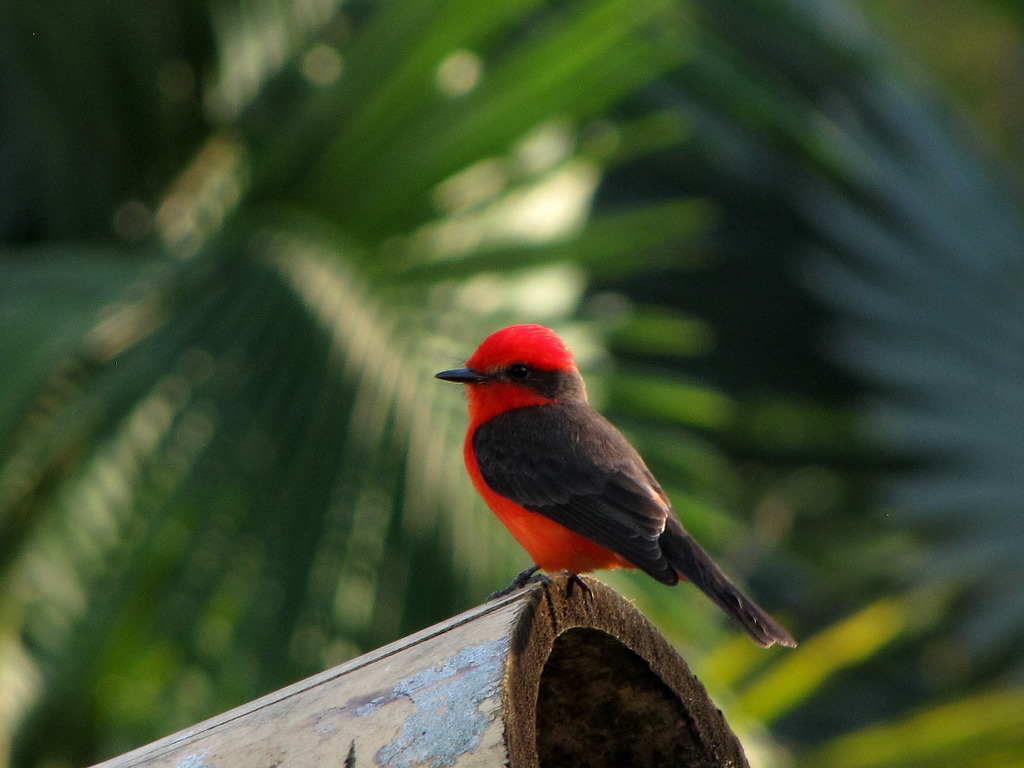
\includegraphics[scale=0.1]{figuras/Petirrojo2} & imagen 1 \\
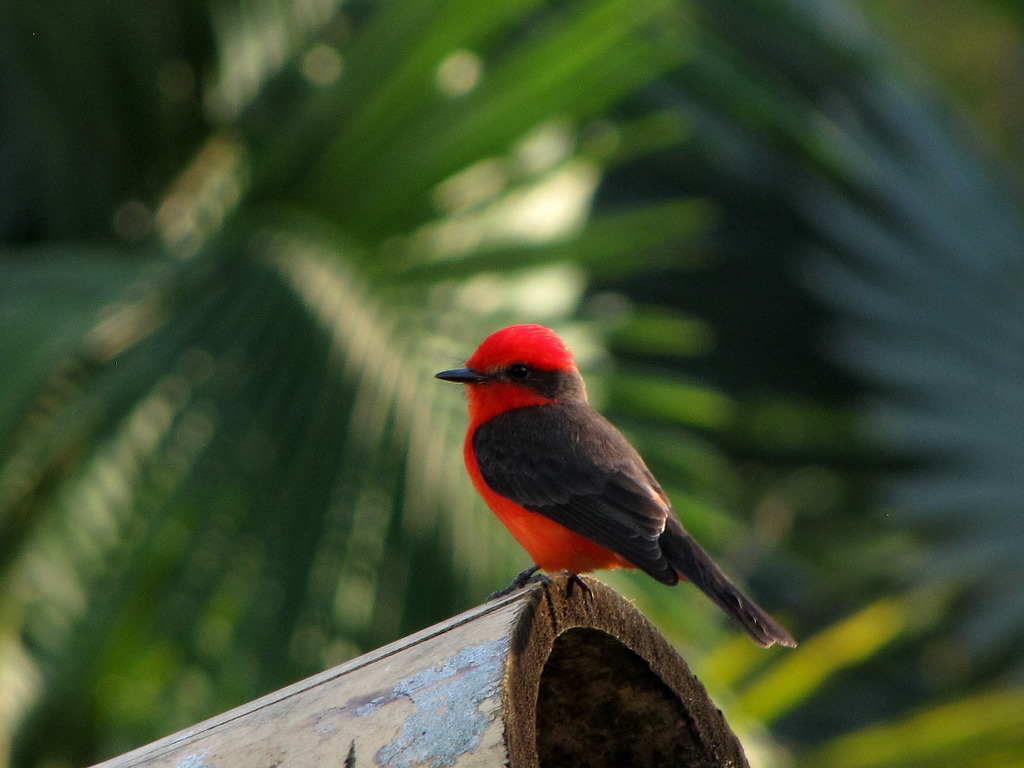
\includegraphics[scale=0.1]{figuras/Petirrojo2} & imagen 2 \\
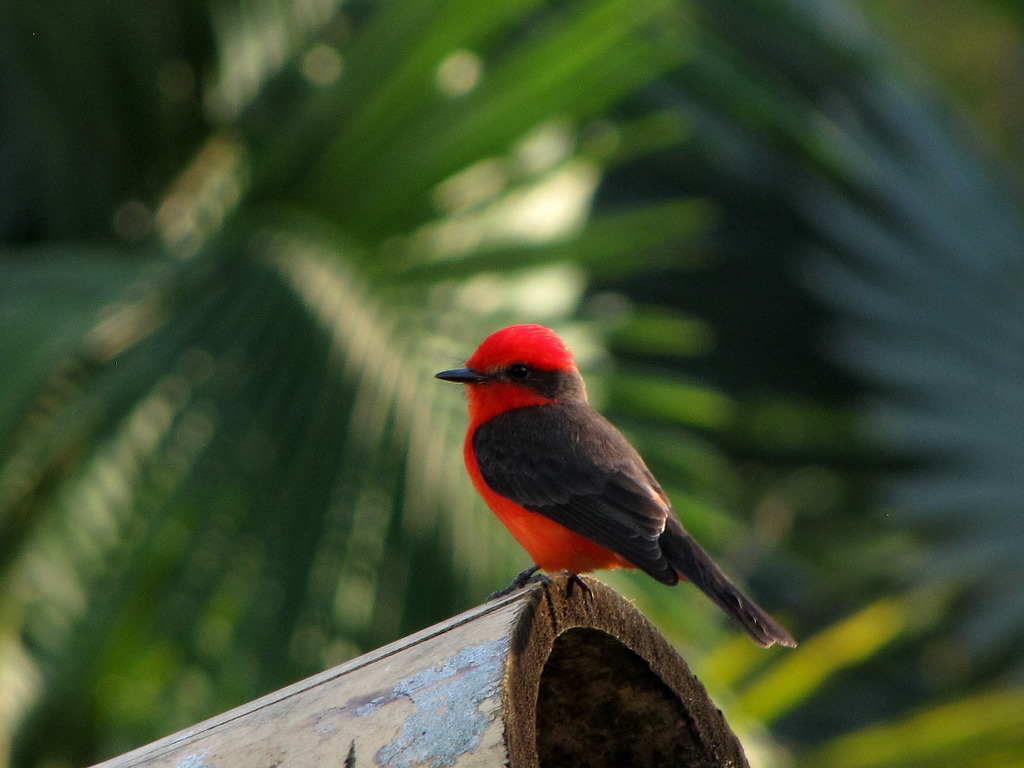
\includegraphics[scale=0.1]{figuras/Petirrojo2} & imagen 3 
\end{tabular}
\caption{Incluir imágenes}
\label{incuirimagen}
\end{table}

\begin{table}[!ht]
\centering
\begin{tabular}{|l|c|r|}
\hline
Lunes & Martes & Miércoles \\
\hline
0     & 0      & 0 \\
\hline
1     & 1      & 1 \\
\hline
\end{tabular}
\caption{tabla con lineas}
\label{incuirimagen}
\end{table}
\newpage
\begin{table}[H]
\centering
\begin{tabular}{|l|c|r|c|}
\hline
Lunes & Martes & Miércoles & Jueves\\
\hline
0     & 0      & 0  & 0\\
\cline{1-2}
1     & 1      & 1  & 0\\
\cline{1-3}
1     & 1      & 1  & 0\\
\hline
\end{tabular}
\caption{tabla con lineas de diferente tamaño}
\label{lineas}
\end{table}
Ejemplo de tablas con lineas 

\begin{table}[H]
\centering
\begin{tabular}{|l|c|r|c|}
\hline
Lunes & Martes & Miércoles & Jueves\\
\hline
0     & 0      & 0  & 0\\
\cline{2-4}
1     & 1      & 1  & 0\\
\cline{2-3}
1     & 1      & 1  & 0\\
\hline
\end{tabular}
\caption{tabla con lineas de diferente tamaño}
\label{lineas}
\end{table}

\subsection{Múltiples columnas}

\begin{table}[H]
\centering
\begin{tabular}{|l|c|r|c|}
\hline
\multicolumn{2}{|c|}{ Enero } & & \\
\hline
\multicolumn{4}{|c|}{ Días de la semana}\\
\hline
 & \multicolumn{3}{|c|}{ Días de la semana 2}\\
\hline
Lunes & Martes & Miércoles & Jueves\\
\hline
0     & 0      & 0  & 0\\
\cline{2-4}
1     & 1      & 1  & 0\\
\cline{2-3}
1     & 1      & 1  & 0\\
\hline
\end{tabular}
\caption{tabla con lineas de diferente tamaño}
\label{lineas}
\end{table}

\section{Tablas con párrafos}

\begin{table}[H]
\centering
\begin{tabular}{|l|p{6cm}|}
\hline
Comando & Descripción \\
\hline
p$\{$Ancho$\}$ & Crea una columna con un ancho fijo. El contenido de esta celda se compone de un párrafo ordinario, sin sangría inicial\\
\hline
m$\{$Ancho$\}$ & Crea una columna con un ancho fijo. El parrafo aparece verticalmente centrado respecto a las columnas vecinas\\
\hline
\end{tabular}
\caption{tabla con parrafos}
\label{lineas}
\end{table}

\begin{table}[H]
\centering
\begin{tabular}{|l|m{6cm}|}
\hline
Comando & Descripción \\
\hline
p$\{$Ancho$\}$ & Crea una columna con un ancho fijo. El contenido de esta celda se compone de un párrafo ordinario, sin sangría inicial\\
\hline
m$\{$Ancho$\}$ & Crea una columna con un ancho fijo. El párrafo aparece verticalmente centrado respecto a las columnas vecinas\\
\hline
\end{tabular}
\caption{tabla con párrafos}
\label{lineas}
\end{table}

\subsection{Escalar una tabla}

\begin{table}[H]
\centering
\scalebox{0.8}{
\begin{tabular}{|l|m{6cm}|}
\hline
Comando & Descripción \\
\hline
p$\{$Ancho$\}$ & Crea una columna con un ancho fijo. El contenido de esta celda se compone de un párrafo ordinario, sin sangría inicial\\
\hline
m$\{$Ancho$\}$ & Crea una columna con un ancho fijo. El párrafo aparece verticalmente centrado respecto a las columnas vecinas\\
\hline
\end{tabular}
}
\caption{tabla escalada}
\label{lineas}
\end{table}

\section{Expresiones matemáticas en tablas}

\begin{table}[H]
\centering
\begin{tabular}{|l|c|c|}
\hline
matemática & $x+1$ & $\lambda$ \\
\hline
ejemplo & $x_{2}$  & $x_{3}$ \\
\hline
$(a+b)^{2}$ & $(a+b)^{3}$ & $(a+b)^{4}$\\
\hline
\end{tabular}
\caption{Usar expresiones matemáticas de forma manual}
\end{table}

\begin{table}[H]
\centering
\begin{tabular}{|>{$}c<{$}|>{$}c<{$}|>{$}c<{$}|}
\hline
x & x+1 & \lambda \\
\hline
x_{1} & x_{2}  & x_{3} \\
\hline
(a+b)^{2} & (a+b)^{3} & (a+b)^{4}\\
\hline
\end{tabular}
\caption{Usar expresiones matemáticas de forma manual}
\end{table}

\begin{table}[H]
\centering
\begin{tabular}{|E|E|E|}
\hline
x & x+1 & \lambda \\
\hline
x_{1} & x_{2}  & x_{3} \\
\hline
(a+b)^{2} & (a+b)^{3} & (a+b)^{4}\\
\hline
\end{tabular}
\caption{Usar expresiones matemáticas de automática}
\end{table}

\section{Tablas largas, paquete longtable}

\begin{longtable}[c]{|ccc|}
Nombre & teléfono & edad \\
Nombre & teléfono & edad \\
Nombre & teléfono & edad \\
Nombre & teléfono & edad \\
Nombre & teléfono & edad \\
Nombre & teléfono & edad \\
Nombre & teléfono & edad \\
Nombre & teléfono & edad \\
Nombre & teléfono & edad \\
Nombre & teléfono & edad \\
A & 12345 & 20 \\
Nombre & teléfono & edad \\
Nombre & teléfono & edad \\
Nombre & teléfono & edad \\
Nombre & teléfono & edad \\
Nombre & teléfono & edad \\
Nombre & teléfono & edad \\
Nombre & teléfono & edad \\
Nombre & teléfono & edad \\
Nombre & teléfono & edad \\
Nombre & teléfono & edad \\
A & 12345 & 20 \\
Nombre & teléfono & edad \\
Nombre & teléfono & edad \\
Nombre & teléfono & edad \\
Nombre & teléfono & edad \\
Nombre & teléfono & edad \\
Nombre & teléfono & edad \\
Nombre & teléfono & edad \\
Nombre & teléfono & edad \\
Nombre & teléfono & edad \\
Nombre & teléfono & edad \\
A & 12345 & 20 \\
Nombre & teléfono & edad \\
Nombre & teléfono & edad \\
Nombre & teléfono & edad \\
Nombre & teléfono & edad \\
Nombre & teléfono & edad \\
Nombre & teléfono & edad \\
Nombre & teléfono & edad \\
Nombre & teléfono & edad \\
Nombre & teléfono & edad \\
Nombre & teléfono & edad \\
A & 12345 & 20 \\
Nombre & teléfono & edad \\
Nombre & teléfono & edad \\
Nombre & teléfono & edad \\
Nombre & teléfono & edad \\
Nombre & teléfono & edad \\
Nombre & teléfono & edad \\
Nombre & teléfono & edad \\
Nombre & teléfono & edad \\
Nombre & teléfono & edad \\
Nombre & teléfono & edad \\
A & 12345 & 20 \\
Nombre & teléfono & edad \\
Nombre & teléfono & edad \\
Nombre & teléfono & edad \\
Nombre & teléfono & edad \\
Nombre & teléfono & edad \\
Nombre & teléfono & edad \\
Nombre & teléfono & edad \\
Nombre & teléfono & edad \\
Nombre & teléfono & edad \\
Nombre & teléfono & edad \\
A & 12345 & 20 \\
Nombre & teléfono & edad \\
Nombre & teléfono & edad \\
Nombre & teléfono & edad \\
Nombre & teléfono & edad \\
Nombre & teléfono & edad \\
Nombre & teléfono & edad \\
Nombre & teléfono & edad \\
Nombre & teléfono & edad \\
Nombre & teléfono & edad \\
Nombre & teléfono & edad \\
A & 12345 & 20 \\
\caption{Tabla larga}
\label{TablaLargaEjempplo}
\end{longtable}

\end{document}
